\chapter{Basic Python}


This book is not intended as a first course in programming.
It will be assumed that the reader has some experience with programming.
Therefore, it will be assumed that certain concepts are already familiar to them, the most basic of which is a mental model for programming that is sometimes called \emph{Sequence, Selection, and Iteration}.

\section{Sequence, Selection, and Iteration}


A recurring theme in this course is the process of moving from \emph{thinking about} code to \emph{writing} code.  We will try to shape the way we think about programs, the way we write programs, and how we go between the two in \emph{both} directions.  That is, we want to have facility with both direct manipulation of code as well as high-level description of programs.\\
A nice model for thinking about (imperative) programming is called Sequence-Selection-Iteration.  It refers to:
1. \textbf{Sequence}: Performing operations one at a time in a specified order.
2. \textbf{Selection}: Using conditional statements such as \texttt{if} to select which operations to execute.
3. \textbf{Iteration}: Repeating some operations using loops or recursion.


In any given programming language, there are usually several mechanisms for selection and iteration, while sequencing is just the default behavior.\\
In fact, you usually have to have special constructions in a language to do something other than performing the given operations in the given order.

\section{Expressions and Evaluation}


Python can do simple arithmetic.  For example, \texttt{2 + 2} is a simple arithmetic \textbf{expression}.
Expressions get \textbf{evaluated} and produce a \textbf{value}.  Some values are numerical like the \texttt{2 + 2} example, but they don’t need to be.
For example, \texttt{5 > 7} is an expression that evaluates to the boolean value \texttt{False}.
Expressions can become more complex by combining many operations and functions.
For example, \texttt{5 * (3 + abs(-12) / 3)} contains four different functions.  Parentheses and the order of operations determine the order that the functions are evaluated.  Recall that in programming the order of operations is also called \textbf{operator precedence}.  In the above example, the functions are executed in the following order: \texttt{abs}, \texttt{/},  \texttt{+}, \texttt{*}.

\section{Variables, Types,  and State}


Imagine you are trying to work out some elaborate math problem without a computer.   It helps to have paper.  You write things down, so that you can use them later.  It's the same in programming.  It often happens that you compute something and want to keep it until later when you will use it.  We often refer to stored information as \textbf{state}.  


We store information in \textbf{variables}.  In Python, a variable is created by an \textbf{assignment} statement.  That is a statement of the form:

\begin{Verbatim}[commandchars=\\\{\}]
\PY{n}{variable\PYZus{}name} \PY{o}{=} \PY{n}{some\PYZus{}value}
\end{Verbatim}



The equals sign is \emph{doing} something (assignment) rather than \emph{describing} something (equality).
The right side of \texttt{=} is an expression that gets evaluated first.  Only later does the assignment happen.
If the left side of the assignment is a variable name that already exist, it is overwritten.
If it doesn’t already exist, it is created.  


The order of evaluation is very important.  Having the right side evaluated first means that assignments like \texttt{x = x + 1} make sense, because the value of \texttt{x} doesn’t change until after \texttt{x + 1} is evaluated.  Incidentally, there is a shorthand for this kind of update: \texttt{x += 1}.  There are similar notations for \texttt{-=}, \texttt{*=}, and \texttt{/=}.


An assignment statement is not expression.  It doesn’t have a value.  This turns out to be useful in avoiding a common bug arising from confusing assignment and equality testing (i.e. \texttt{x == y}).  However, multiple assignment like \texttt{x = y = 1} does work as you would expect it to, setting both \texttt{x} and \texttt{y} to \texttt{1}.


Variables are  just names.  Every name is associated with some piece of data, called an object.\\
The name is a string of characters and it is mapped to an object.
The name of a variable, by itself, is treated as an expression that evaluates to whatever object it is mapped to.
This mapping of strings to objects is often depicted using boxes to represent the objects and arrows to show the mapping.


Every object has a \textbf{type}.  The type often determines what you can do with the variable.  The so-called \textbf{atomic types} in Python are \emph{integers}, \emph{floats}, and \emph{booleans}, but any interesting program will contain variables of many other types as well.  You can inspect the type of a variable using the \texttt{type()} function.  In Python, the word \emph{type} and \emph{class} mean the same thing (most of the time).


The difference between a variable and the \textbf{object} it represents can get lost in our common speech because the variable is usually acting as the \emph{name} of the object.  There are some times when it's useful to be clear about the difference, in particular when copying objects.  You might want to try some examples of copying objects from one variable to another.  Does changing one of them affect the other?

\begin{Verbatim}[commandchars=\\\{\}]
\PY{n}{x} \PY{o}{=} \PY{l+m+mi}{5}
\PY{n}{y} \PY{o}{=} \PY{l+m+mf}{3.2}
\PY{n}{z} \PY{o}{=} \PY{k+kc}{True}
\PY{n+nb}{print}\PY{p}{(}\PY{l+s+s2}{\PYZdq{}}\PY{l+s+s2}{x has type}\PY{l+s+s2}{\PYZdq{}}\PY{p}{,} \PY{n+nb}{type}\PY{p}{(}\PY{n}{x}\PY{p}{)}\PY{p}{)}
\PY{n+nb}{print}\PY{p}{(}\PY{l+s+s2}{\PYZdq{}}\PY{l+s+s2}{y has type}\PY{l+s+s2}{\PYZdq{}}\PY{p}{,} \PY{n+nb}{type}\PY{p}{(}\PY{n}{y}\PY{p}{)}\PY{p}{)}
\PY{n+nb}{print}\PY{p}{(}\PY{l+s+s2}{\PYZdq{}}\PY{l+s+s2}{z has type}\PY{l+s+s2}{\PYZdq{}}\PY{p}{,} \PY{n+nb}{type}\PY{p}{(}\PY{n}{z}\PY{p}{)}\PY{p}{)}
\end{Verbatim}



You should think of an object as having three things: an \emph{identity}, a \emph{type}, and a \emph{value}.
Its identity cannot change.  It can be used to see if two objects are actually the same object with the \texttt{is} keyword.
For example, consider the following code.

\begin{Verbatim}[commandchars=\\\{\}]
\PY{n}{x} \PY{o}{=} \PY{p}{[}\PY{l+m+mi}{1}\PY{p}{,} \PY{l+m+mi}{2}\PY{p}{,} \PY{l+m+mi}{3}\PY{p}{]}
\PY{n}{y} \PY{o}{=} \PY{n}{x}
\PY{n}{z} \PY{o}{=} \PY{p}{[}\PY{l+m+mi}{1}\PY{p}{,} \PY{l+m+mi}{2}\PY{p}{,} \PY{l+m+mi}{3}\PY{p}{]}

\PY{n+nb}{print}\PY{p}{(}\PY{n}{x} \PY{o+ow}{is} \PY{n}{y}\PY{p}{)}
\PY{n+nb}{print}\PY{p}{(}\PY{n}{x} \PY{o+ow}{is} \PY{n}{z}\PY{p}{)}
\PY{n+nb}{print}\PY{p}{(}\PY{n}{x} \PY{o}{==} \PY{n}{z}\PY{p}{)}
\end{Verbatim}



An object cannot change its identity.
In Python, you also cannot change the type of an object.
You can reassign a variable to point to different object of a different type, but that's not the same thing.
There are several functions that may seem to be changing the types of objects, but they are really just creating a new object from the old.

\begin{Verbatim}[commandchars=\\\{\}]
\PY{n}{x} \PY{o}{=} \PY{l+m+mi}{2}
\PY{n+nb}{print}\PY{p}{(}\PY{l+s+s2}{\PYZdq{}}\PY{l+s+s2}{x =}\PY{l+s+s2}{\PYZdq{}}\PY{p}{,} \PY{n}{x}\PY{p}{)}
\PY{n+nb}{print}\PY{p}{(}\PY{l+s+s2}{\PYZdq{}}\PY{l+s+s2}{float(x) =}\PY{l+s+s2}{\PYZdq{}}\PY{p}{,} \PY{n+nb}{float}\PY{p}{(}\PY{n}{x}\PY{p}{)}\PY{p}{)}
\PY{n+nb}{print}\PY{p}{(}\PY{l+s+s2}{\PYZdq{}}\PY{l+s+s2}{x still has type}\PY{l+s+s2}{\PYZdq{}}\PY{p}{,} \PY{n+nb}{type}\PY{p}{(}\PY{n}{x}\PY{p}{)}\PY{p}{)}

\PY{n+nb}{print}\PY{p}{(}\PY{l+s+s2}{\PYZdq{}}\PY{l+s+s2}{Overwriting x.}\PY{l+s+s2}{\PYZdq{}}\PY{p}{)}
\PY{n}{x} \PY{o}{=} \PY{n+nb}{float}\PY{p}{(}\PY{n}{x}\PY{p}{)}
\PY{n+nb}{print}\PY{p}{(}\PY{l+s+s2}{\PYZdq{}}\PY{l+s+s2}{Now, x has type}\PY{l+s+s2}{\PYZdq{}}\PY{p}{,} \PY{n+nb}{type}\PY{p}{(}\PY{n}{x}\PY{p}{)}\PY{p}{)}
\end{Verbatim}



You can do more elaborate things as well.

\begin{Verbatim}[commandchars=\\\{\}]
\PY{n}{numstring} \PY{o}{=} \PY{l+s+s2}{\PYZdq{}}\PY{l+s+s2}{3.1415926}\PY{l+s+s2}{\PYZdq{}}
\PY{n}{y} \PY{o}{=} \PY{n+nb}{float}\PY{p}{(}\PY{n}{numstring}\PY{p}{)}
\PY{n+nb}{print}\PY{p}{(}\PY{l+s+s2}{\PYZdq{}}\PY{l+s+s2}{y has type}\PY{l+s+s2}{\PYZdq{}}\PY{p}{,} \PY{n+nb}{type}\PY{p}{(}\PY{n}{y}\PY{p}{)}\PY{p}{)}

\PY{n}{best\PYZus{}number} \PY{o}{=} \PY{l+m+mi}{73}
\PY{n}{x} \PY{o}{=} \PY{n+nb}{str}\PY{p}{(}\PY{n}{best\PYZus{}number}\PY{p}{)}
\PY{n+nb}{print}\PY{p}{(}\PY{l+s+s2}{\PYZdq{}}\PY{l+s+s2}{x has type}\PY{l+s+s2}{\PYZdq{}}\PY{p}{,} \PY{n+nb}{type}\PY{p}{(}\PY{n}{x}\PY{p}{)}\PY{p}{)}

\PY{n}{thisworks} \PY{o}{=} \PY{n+nb}{float}\PY{p}{(}\PY{l+s+s2}{\PYZdq{}}\PY{l+s+s2}{inf}\PY{l+s+s2}{\PYZdq{}}\PY{p}{)}
\PY{n+nb}{print}\PY{p}{(}\PY{l+s+s2}{\PYZdq{}}\PY{l+s+s2}{float(}\PY{l+s+se}{\PYZbs{}\PYZsq{}}\PY{l+s+s2}{inf}\PY{l+s+se}{\PYZbs{}\PYZsq{}}\PY{l+s+s2}{) has type}\PY{l+s+s2}{\PYZdq{}}\PY{p}{,} \PY{n+nb}{type}\PY{p}{(}\PY{n}{thisworks}\PY{p}{)}\PY{p}{)}
\PY{n}{infinity\PYZus{}plus\PYZus{}one} \PY{o}{=} \PY{n+nb}{float}\PY{p}{(}\PY{l+s+s1}{\PYZsq{}}\PY{l+s+s1}{inf}\PY{l+s+s1}{\PYZsq{}}\PY{p}{)} \PY{o}{+} \PY{l+m+mi}{1}
\end{Verbatim}



This last example introduced a new type, that of a \textbf{string}.  A string is a sequence of characters.  In Python, there is no special class for a single character (as in C for example).
If you want a single character, you use a string of length one.


The value of an object may or may not be changed, depending on the type of object.
If the value can be changed, we say that the object is \textbf{mutable}.
If it cannot be changed, we say that the object is \textbf{immutable}.
For example, strings are immutable.  If you want to change a string, for example, by converting it to lowercase, then you will be creating a new string.

\section{Collections}


The next five most important types in Python are strings, lists, tuples, dictionaries, and sets.  We call these collections as each can be used for storing a collection of things.  We will see many other examples of collections in this course.

\subsection{Strings  (\texttt{str})}


\textbf{Strings} are sequences of characters and can be used to store text of all kinds.  Note that you can \textbf{concatenate} strings to create a new string using the plus sign.  You can also access individual characters using square brackets and an \textbf{index}.  The name of the class for strings is \texttt{str}.  You can often turn other objects into strings.

\begin{Verbatim}[commandchars=\\\{\}]
\PY{n}{s} \PY{o}{=} \PY{l+s+s2}{\PYZdq{}}\PY{l+s+s2}{Hello, }\PY{l+s+s2}{\PYZdq{}}
\PY{n}{t} \PY{o}{=} \PY{l+s+s2}{\PYZdq{}}\PY{l+s+s2}{World.}\PY{l+s+s2}{\PYZdq{}}
\PY{n}{u} \PY{o}{=} \PY{n}{s} \PY{o}{+} \PY{n}{t}
\PY{n+nb}{print}\PY{p}{(}\PY{n+nb}{type}\PY{p}{(}\PY{n}{u}\PY{p}{)}\PY{p}{)}
\PY{n+nb}{print}\PY{p}{(}\PY{n}{u}\PY{p}{)}
\PY{n+nb}{print}\PY{p}{(}\PY{n}{u}\PY{p}{[}\PY{l+m+mi}{9}\PY{p}{]}\PY{p}{)}
\PY{n}{n} \PY{o}{=} \PY{n+nb}{str}\PY{p}{(}\PY{l+m+mi}{9876}\PY{p}{)}
\PY{n+nb}{print}\PY{p}{(}\PY{n}{n}\PY{p}{[}\PY{l+m+mi}{2}\PY{p}{]}\PY{p}{)}
\end{Verbatim}


\subsection{Lists (\texttt{list})}


\textbf{Lists} are ordered sequences of objects.  The objects do not have to be the same type.  They are indicated by square brackets and the \textbf{elements} of the list are separated by commas.  You can append an item to the end of a list \texttt{L} by using the command \texttt{L.append(newitem)}.
It is possible to index into a list exactly as we did with strings.

\begin{Verbatim}[commandchars=\\\{\}]
\PY{n}{L} \PY{o}{=} \PY{p}{[}\PY{l+m+mi}{1}\PY{p}{,}\PY{l+m+mi}{2}\PY{p}{,}\PY{l+m+mi}{3}\PY{p}{,}\PY{l+m+mi}{4}\PY{p}{,}\PY{l+m+mi}{5}\PY{p}{,}\PY{l+m+mi}{6}\PY{p}{]}
\PY{n+nb}{print}\PY{p}{(}\PY{n+nb}{type}\PY{p}{(}\PY{n}{L}\PY{p}{)}\PY{p}{)}
\end{Verbatim}



Here is a common visual representation of the list.


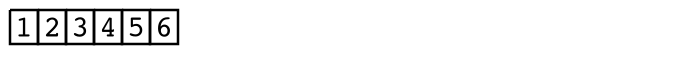
\includegraphics[width=\textwidth]{./figures/list_example01.png}

\begin{Verbatim}[commandchars=\\\{\}]
\PY{n}{L}\PY{o}{.}\PY{n}{append}\PY{p}{(}\PY{l+m+mi}{100}\PY{p}{)}
\end{Verbatim}



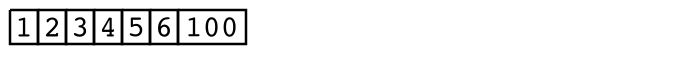
\includegraphics[width=\textwidth]{./figures/list_example02.png}

\subsection{Tuples (\texttt{tuple})}


\textbf{Tuples} are also ordered sequences of objects, but unlike lists, they are immutable.  You can access the items but you can’t change what items are in the tuple after you create it.  For example, trying to \texttt{append} raises an exception.

\begin{Verbatim}[commandchars=\\\{\}]
\PY{n}{t} \PY{o}{=} \PY{p}{(}\PY{l+m+mi}{1}\PY{p}{,} \PY{l+m+mi}{2}\PY{p}{,} \PY{l+s+s2}{\PYZdq{}}\PY{l+s+s2}{skip a few}\PY{l+s+s2}{\PYZdq{}}\PY{p}{,} \PY{l+m+mi}{99}\PY{p}{,} \PY{l+m+mi}{100}\PY{p}{)}
\PY{n+nb}{print}\PY{p}{(}\PY{n+nb}{type}\PY{p}{(}\PY{n}{t}\PY{p}{)}\PY{p}{)}
\PY{n+nb}{print}\PY{p}{(}\PY{n}{t}\PY{p}{)}
\PY{n+nb}{print}\PY{p}{(}\PY{n}{t}\PY{p}{[}\PY{l+m+mi}{4}\PY{p}{]}\PY{p}{)}
\PY{n}{t}\PY{o}{.}\PY{n}{append}\PY{p}{(}\PY{l+m+mi}{101}\PY{p}{)}
\end{Verbatim}


\subsection{Dictionaries (\texttt{dict})}


\textbf{Dictionaries} store \emph{key-value} pairs.  That is, every element of a dictionary has two parts, a \textbf{key} and a \textbf{value}.  If you have the key, you can get the value.  The name comes from the idea that in a real dictionary (book), a word (the key) allows you to find its definition (the value).  Notice that the keys can be different types, but they must be immutable types such as atomic types, tuples, or strings.  The reason for this requirement is that we will determine where to store something using the key.  If the key changes, we will look in the wrong place when it's time to look it up again.


Dictionaries are also known as maps,  \textbf{mappings}, or hash tables.  We will go deep into how these are constructed later in the course.
A dictionary doesn't have a fixed order.

\begin{Verbatim}[commandchars=\\\{\}]
\PY{n}{d} \PY{o}{=} \PY{n+nb}{dict}\PY{p}{(}\PY{p}{)}
\PY{n}{d}\PY{p}{[}\PY{l+m+mi}{2}\PY{p}{]} \PY{o}{=} \PY{l+s+s2}{\PYZdq{}}\PY{l+s+s2}{two}\PY{l+s+s2}{\PYZdq{}}
\PY{n}{d}\PY{p}{[}\PY{l+m+mi}{5}\PY{p}{]} \PY{o}{=} \PY{l+s+s2}{\PYZdq{}}\PY{l+s+s2}{five}\PY{l+s+s2}{\PYZdq{}}
\PY{n}{d}\PY{p}{[}\PY{l+s+s2}{\PYZdq{}}\PY{l+s+s2}{pi}\PY{l+s+s2}{\PYZdq{}}\PY{p}{]} \PY{o}{=} \PY{l+m+mf}{3.1415926}

\PY{n+nb}{print}\PY{p}{(}\PY{n}{d}\PY{p}{)}
\PY{n+nb}{print}\PY{p}{(}\PY{n}{d}\PY{p}{[}\PY{l+s+s2}{\PYZdq{}}\PY{l+s+s2}{pi}\PY{l+s+s2}{\PYZdq{}}\PY{p}{]}\PY{p}{)}
\end{Verbatim}


\subsection{Sets (\texttt{set})}


\textbf{Sets} correspond to our notion of sets in math.  They are collections of objects without duplicates.  We use curly braces to denote them and commas to separate elements.  As with dictionaries, a set has no fixed ordering.  We say that sets and dictionaries are \textbf{nonsequential collections}.


Be careful that empty braces \texttt{{}} indicates an empty dictionary and not an empty set.  Here is an example of a newly created set.  Some items are added.  Notice that the duplicates have no effect on the value as its printed.

\begin{Verbatim}[commandchars=\\\{\}]
\PY{n}{s} \PY{o}{=} \PY{p}{\PYZob{}}\PY{l+m+mi}{2}\PY{p}{,}\PY{l+m+mi}{1}\PY{p}{\PYZcb{}}
\PY{n+nb}{print}\PY{p}{(}\PY{n+nb}{type}\PY{p}{(}\PY{n}{s}\PY{p}{)}\PY{p}{)}
\PY{n}{s}\PY{o}{.}\PY{n}{add}\PY{p}{(}\PY{l+m+mi}{3}\PY{p}{)}
\PY{n}{s}\PY{o}{.}\PY{n}{add}\PY{p}{(}\PY{l+m+mi}{2}\PY{p}{)}
\PY{n}{s}\PY{o}{.}\PY{n}{add}\PY{p}{(}\PY{l+m+mi}{2}\PY{p}{)}
\PY{n}{s}\PY{o}{.}\PY{n}{add}\PY{p}{(}\PY{l+m+mi}{2}\PY{p}{)}
\PY{n+nb}{print}\PY{p}{(}\PY{n}{s}\PY{p}{)}
\end{Verbatim}


\section{Some common things to do with collections}


There are several operations that can be performed on any of the collections classes (and indeed often on many other types objects).


You can find the number of elements in the collection (the \textbf{length}) using \texttt{len}.

\begin{Verbatim}[commandchars=\\\{\}]
\PY{n}{a} \PY{o}{=} \PY{l+s+s2}{\PYZdq{}}\PY{l+s+s2}{a string}\PY{l+s+s2}{\PYZdq{}}
\PY{n}{b} \PY{o}{=} \PY{p}{[}\PY{l+s+s2}{\PYZdq{}}\PY{l+s+s2}{my}\PY{l+s+s2}{\PYZdq{}}\PY{p}{,} \PY{l+s+s2}{\PYZdq{}}\PY{l+s+s2}{second}\PY{l+s+s2}{\PYZdq{}}\PY{p}{,} \PY{l+s+s2}{\PYZdq{}}\PY{l+s+s2}{favorite}\PY{l+s+s2}{\PYZdq{}}\PY{p}{,} \PY{l+s+s2}{\PYZdq{}}\PY{l+s+s2}{list}\PY{l+s+s2}{\PYZdq{}}\PY{p}{]}
\PY{n}{c} \PY{o}{=} \PY{p}{(}\PY{l+m+mi}{1}\PY{p}{,} \PY{l+s+s2}{\PYZdq{}}\PY{l+s+s2}{tuple}\PY{l+s+s2}{\PYZdq{}}\PY{p}{)}
\PY{n}{d} \PY{o}{=} \PY{p}{\PYZob{}}\PY{l+s+s1}{\PYZsq{}}\PY{l+s+s1}{a}\PY{l+s+s1}{\PYZsq{}}\PY{p}{:} \PY{l+s+s1}{\PYZsq{}}\PY{l+s+s1}{b}\PY{l+s+s1}{\PYZsq{}}\PY{p}{,} \PY{l+s+s1}{\PYZsq{}}\PY{l+s+s1}{b}\PY{l+s+s1}{\PYZsq{}}\PY{p}{:} \PY{l+m+mi}{2}\PY{p}{,} \PY{l+s+s1}{\PYZsq{}}\PY{l+s+s1}{c}\PY{l+s+s1}{\PYZsq{}}\PY{p}{:} \PY{k+kc}{False}\PY{p}{\PYZcb{}}
\PY{n}{e} \PY{o}{=} \PY{p}{\PYZob{}}\PY{l+m+mi}{1}\PY{p}{,}\PY{l+m+mi}{2}\PY{p}{,}\PY{l+m+mi}{3}\PY{p}{,}\PY{l+m+mi}{4}\PY{p}{,}\PY{l+m+mi}{4}\PY{p}{,}\PY{l+m+mi}{4}\PY{p}{,}\PY{l+m+mi}{4}\PY{p}{,}\PY{l+m+mi}{2}\PY{p}{,}\PY{l+m+mi}{2}\PY{p}{,}\PY{l+m+mi}{2}\PY{p}{,}\PY{l+m+mi}{1}\PY{p}{\PYZcb{}}

\PY{n+nb}{print}\PY{p}{(}\PY{n+nb}{len}\PY{p}{(}\PY{n}{a}\PY{p}{)}\PY{p}{,} \PY{n+nb}{len}\PY{p}{(}\PY{n}{b}\PY{p}{)}\PY{p}{,} \PY{n+nb}{len}\PY{p}{(}\PY{n}{c}\PY{p}{)}\PY{p}{,} \PY{n+nb}{len}\PY{p}{(}\PY{n}{d}\PY{p}{)}\PY{p}{,} \PY{n+nb}{len}\PY{p}{(}\PY{n}{e}\PY{p}{)}\PY{p}{)}
\end{Verbatim}



For the sequential types (lists, tuples, and strings), you can \textbf{slice} a subsequence of indices using square brackets and a colon as in the following examples.  The range of indices is half open in that the slice will start with the first index and proceed up to but not including the last index.  Negative indices count backwards from the end.  Leaving out the first index is the same as starting at 0.  Leaving out the second index will continue the slice until the end of the sequence.


\textbf{Important}: slicing a sequence creates a new object.  That means a big slice will do a lot of copying.  It's really easy to write inefficient code this way.

\begin{Verbatim}[commandchars=\\\{\}]
\PY{n}{a} \PY{o}{=} \PY{l+s+s2}{\PYZdq{}}\PY{l+s+s2}{a string}\PY{l+s+s2}{\PYZdq{}}
\PY{n}{b} \PY{o}{=} \PY{p}{[}\PY{l+s+s2}{\PYZdq{}}\PY{l+s+s2}{my}\PY{l+s+s2}{\PYZdq{}}\PY{p}{,} \PY{l+s+s2}{\PYZdq{}}\PY{l+s+s2}{second}\PY{l+s+s2}{\PYZdq{}}\PY{p}{,} \PY{l+s+s2}{\PYZdq{}}\PY{l+s+s2}{favorite}\PY{l+s+s2}{\PYZdq{}}\PY{p}{,} \PY{l+s+s2}{\PYZdq{}}\PY{l+s+s2}{list}\PY{l+s+s2}{\PYZdq{}}\PY{p}{]}
\PY{n}{c} \PY{o}{=} \PY{p}{(}\PY{l+m+mi}{1}\PY{p}{,} \PY{l+m+mi}{2}\PY{p}{,}\PY{l+m+mi}{3}\PY{p}{,}\PY{l+s+s2}{\PYZdq{}}\PY{l+s+s2}{tuple}\PY{l+s+s2}{\PYZdq{}}\PY{p}{)}
\PY{n+nb}{print}\PY{p}{(}\PY{n}{a}\PY{p}{[}\PY{l+m+mi}{3}\PY{p}{:}\PY{l+m+mi}{7}\PY{p}{]}\PY{p}{)}
\PY{n+nb}{print}\PY{p}{(}\PY{n}{a}\PY{p}{[}\PY{l+m+mi}{1}\PY{p}{:}\PY{o}{\PYZhy{}}\PY{l+m+mi}{2}\PY{p}{]}\PY{p}{)}
\PY{n+nb}{print}\PY{p}{(}\PY{n}{b}\PY{p}{[}\PY{l+m+mi}{1}\PY{p}{:}\PY{p}{]}\PY{p}{)}
\PY{n+nb}{print}\PY{p}{(}\PY{n}{c}\PY{p}{[}\PY{p}{:}\PY{l+m+mi}{2}\PY{p}{]}\PY{p}{)}
\end{Verbatim}


\section{Iterating over a collection}


It is very common to want to loop over a collection.
The pythonic way of doing iteration is with a \texttt{for} loop.


The syntax is shown in the following examples.

\begin{Verbatim}[commandchars=\\\{\}]
\PY{n}{mylist} \PY{o}{=} \PY{p}{[}\PY{l+m+mi}{1}\PY{p}{,}\PY{l+m+mi}{3}\PY{p}{,}\PY{l+m+mi}{5}\PY{p}{]}
\PY{n}{mytuple} \PY{o}{=} \PY{p}{(}\PY{l+m+mi}{1}\PY{p}{,} \PY{l+m+mi}{2}\PY{p}{,} \PY{l+s+s1}{\PYZsq{}}\PY{l+s+s1}{skip a few}\PY{l+s+s1}{\PYZsq{}}\PY{p}{,} \PY{l+m+mi}{99}\PY{p}{,} \PY{l+m+mi}{100}\PY{p}{)}
\PY{n}{myset} \PY{o}{=} \PY{p}{\PYZob{}}\PY{l+s+s1}{\PYZsq{}}\PY{l+s+s1}{a}\PY{l+s+s1}{\PYZsq{}}\PY{p}{,} \PY{l+s+s1}{\PYZsq{}}\PY{l+s+s1}{b}\PY{l+s+s1}{\PYZsq{}}\PY{p}{,} \PY{l+s+s1}{\PYZsq{}}\PY{l+s+s1}{z}\PY{l+s+s1}{\PYZsq{}}\PY{p}{\PYZcb{}}
\PY{n}{mystring} \PY{o}{=} \PY{l+s+s1}{\PYZsq{}}\PY{l+s+s1}{abracadabra}\PY{l+s+s1}{\PYZsq{}}
\PY{n}{mydict} \PY{o}{=} \PY{p}{\PYZob{}}\PY{l+s+s1}{\PYZsq{}}\PY{l+s+s1}{a}\PY{l+s+s1}{\PYZsq{}}\PY{p}{:} \PY{l+m+mi}{96}\PY{p}{,} \PY{l+s+s1}{\PYZsq{}}\PY{l+s+s1}{b}\PY{l+s+s1}{\PYZsq{}}\PY{p}{:} \PY{l+m+mi}{97}\PY{p}{,} \PY{l+s+s1}{\PYZsq{}}\PY{l+s+s1}{c}\PY{l+s+s1}{\PYZsq{}}\PY{p}{:} \PY{l+m+mi}{98}\PY{p}{\PYZcb{}}

\PY{k}{for} \PY{n}{item} \PY{o+ow}{in} \PY{n}{mylist}\PY{p}{:}
    \PY{n+nb}{print}\PY{p}{(}\PY{n}{item}\PY{p}{)}

\PY{k}{for} \PY{n}{item} \PY{o+ow}{in} \PY{n}{mytuple}\PY{p}{:}
    \PY{n+nb}{print}\PY{p}{(}\PY{n}{item}\PY{p}{)}

\PY{k}{for} \PY{n}{element} \PY{o+ow}{in} \PY{n}{myset}\PY{p}{:}
    \PY{n+nb}{print}\PY{p}{(}\PY{n}{element}\PY{p}{)}

\PY{k}{for} \PY{n}{character} \PY{o+ow}{in} \PY{n}{mystring}\PY{p}{:}
    \PY{n+nb}{print}\PY{p}{(}\PY{n}{character}\PY{p}{)}

\PY{k}{for} \PY{n}{key} \PY{o+ow}{in} \PY{n}{mydict}\PY{p}{:}
    \PY{n+nb}{print}\PY{p}{(}\PY{n}{key}\PY{p}{)}

\PY{k}{for} \PY{n}{key}\PY{p}{,} \PY{n}{value} \PY{o+ow}{in} \PY{n}{mydict}\PY{o}{.}\PY{n}{items}\PY{p}{(}\PY{p}{)}\PY{p}{:}
    \PY{n+nb}{print}\PY{p}{(}\PY{n}{key}\PY{p}{,} \PY{n}{value}\PY{p}{)}

\PY{k}{for} \PY{n}{value} \PY{o+ow}{in} \PY{n}{mydict}\PY{o}{.}\PY{n}{values}\PY{p}{(}\PY{p}{)}\PY{p}{:}
    \PY{n+nb}{print}\PY{p}{(}\PY{n}{value}\PY{p}{)}
\end{Verbatim}



There is class called \texttt{range} to represent a sequence of numbers that behaves like a collection.
It is often used in for loops as follows.

\begin{Verbatim}[commandchars=\\\{\}]
\PY{k}{for} \PY{n}{i} \PY{o+ow}{in} \PY{n+nb}{range}\PY{p}{(}\PY{l+m+mi}{10}\PY{p}{)}\PY{p}{:}
    \PY{n}{j} \PY{o}{=} \PY{l+m+mi}{10} \PY{o}{*} \PY{n}{i} \PY{o}{+} \PY{l+m+mi}{1}
    \PY{n+nb}{print}\PY{p}{(}\PY{n}{j}\PY{p}{,}\PY{p}{)}
\end{Verbatim}


\section{Other Forms of Control Flow}


\textbf{Control flow} refers to the commands in a language that affect the order or what operations are executed.
The \texttt{for} loops from the previous section are classic examples if this.  The other basic forms of control flow are \texttt{if} statements, \texttt{while} loops,  \texttt{try} blocks, and function calls.  We’ll cover each briefly and refer the reader to the python documentation for more detailed info.


An \texttt{if} statement in its simplest form evaluates an expression and tries to interpret it as a boolean.  This expression is referred to as a predicate.  If the predicate evaluates to \texttt{True}, then a block of code is executed.  Otherwise, the code is not executed.  This is the \emph{selection} of sequence, selection, and iteration.  Here is an example.

\begin{Verbatim}[commandchars=\\\{\}]
\PY{k}{if} \PY{l+m+mi}{3} \PY{o}{+} \PY{l+m+mi}{3} \PY{o}{\PYZlt{}} \PY{l+m+mi}{7}\PY{p}{:}
    \PY{n+nb}{print}\PY{p}{(}\PY{l+s+s2}{\PYZdq{}}\PY{l+s+s2}{This should be printed.}\PY{l+s+s2}{\PYZdq{}}\PY{p}{)}

\PY{k}{if} \PY{l+m+mi}{2} \PY{o}{*}\PY{o}{*} \PY{l+m+mi}{8} \PY{o}{!=} \PY{l+m+mi}{256}\PY{p}{:}
    \PY{n+nb}{print}\PY{p}{(}\PY{l+s+s2}{\PYZdq{}}\PY{l+s+s2}{This should not be printed.}\PY{l+s+s2}{\PYZdq{}}\PY{p}{)}
\end{Verbatim}



An \texttt{if} statement can also include an \texttt{else} clause.  This is a second block of code that executes if the predicate evaluates to \texttt{False}.

\begin{Verbatim}[commandchars=\\\{\}]
\PY{k}{if} \PY{k+kc}{False}\PY{p}{:}
    \PY{n+nb}{print}\PY{p}{(}\PY{l+s+s2}{\PYZdq{}}\PY{l+s+s2}{This is bad.}\PY{l+s+s2}{\PYZdq{}}\PY{p}{)}
\PY{k}{else}\PY{p}{:}
    \PY{n+nb}{print}\PY{p}{(}\PY{l+s+s2}{\PYZdq{}}\PY{l+s+s2}{This will print.}\PY{l+s+s2}{\PYZdq{}}\PY{p}{)}
\end{Verbatim}



A \texttt{while} loop also has a predicate.  It is evaluated at the top of a block of code.  If it evaluates to \texttt{True}, then the block is executed and then it repeats.  The repetition continues until the predicate evaluate to \texttt{False} or until the code reaches a \texttt{break} statement.

\begin{Verbatim}[commandchars=\\\{\}]
\PY{n}{x} \PY{o}{=} \PY{l+m+mi}{1}
\PY{k}{while} \PY{n}{x} \PY{o}{\PYZlt{}} \PY{l+m+mi}{128}\PY{p}{:}
    \PY{n+nb}{print}\PY{p}{(}\PY{n}{x}\PY{p}{)}
    \PY{n}{x} \PY{o}{=} \PY{n}{x} \PY{o}{*} \PY{l+m+mi}{2}
\end{Verbatim}



A \texttt{try} block is the way to catch and recover from errors while a program is running.  If you have some code that may cause an error, but you don’t want it to crash your program, you can put the code in a \texttt{try} block.  Then, you can \emph{catch} the error (also known as an \textbf{exception}) and deal with it.  A simple example might be a case where you want to convert some number to a \texttt{float}.  Many types of objects can be converted to \texttt{float}, but many cannot.  If we simply try to do the conversion and it works, everything is fine.  Otherwise, if there is a \texttt{ValueError}, we can do something else instead.  

\begin{Verbatim}[commandchars=\\\{\}]
\PY{n}{x} \PY{o}{=} \PY{l+s+s2}{\PYZdq{}}\PY{l+s+s2}{not a number}\PY{l+s+s2}{\PYZdq{}}
\PY{k}{try}\PY{p}{:}
    \PY{n}{f} \PY{o}{=} \PY{n+nb}{float}\PY{p}{(}\PY{n}{x}\PY{p}{)}
\PY{k}{except} \PY{n+ne}{ValueError}\PY{p}{:}
    \PY{n+nb}{print}\PY{p}{(}\PY{l+s+s2}{\PYZdq{}}\PY{l+s+s2}{You can’t do that!}\PY{l+s+s2}{\PYZdq{}}\PY{p}{)}
\end{Verbatim}



A function also changes the control flow.  In Python, you define a function with the \texttt{def} keyword.  This keyword creates an object to store the block of code.  The parameters for the function are listed in parentheses after the function name.  The \texttt{return} statement causes the control flow to revert back to where the function was called and determines the value of the function call.  

\begin{Verbatim}[commandchars=\\\{\}]
\PY{k}{def} \PY{n+nf}{foo}\PY{p}{(}\PY{n}{x}\PY{p}{,} \PY{n}{y}\PY{p}{)}\PY{p}{:}
    \PY{k}{return} \PY{l+m+mi}{8} \PY{o}{*} \PY{n}{x} \PY{o}{+} \PY{n}{y}

\PY{n+nb}{print}\PY{p}{(}\PY{n}{foo}\PY{p}{(}\PY{l+m+mi}{2}\PY{p}{,} \PY{l+m+mi}{1}\PY{p}{)}\PY{p}{)}
\PY{n+nb}{print}\PY{p}{(}\PY{n}{foo}\PY{p}{(}\PY{l+s+s2}{\PYZdq{}}\PY{l+s+s2}{Na}\PY{l+s+s2}{\PYZdq{}}\PY{p}{,} \PY{l+s+s2}{\PYZdq{}}\PY{l+s+s2}{ batman}\PY{l+s+s2}{\PYZdq{}}\PY{p}{)}\PY{p}{)}
\end{Verbatim}



Notice that there is no requirement that we specify the types of objects a function expects for its arguments.  This is very convenient, because it means that we can use the same function to operate on different types of objects (as in the example above).  If we define a function twice, even if we change the parameters, the first will be overwritten by the second.  This is exactly the same as assigning to a variable twice.  The name of a function is just a name; it refers to an object (the function).  Functions can be treated like any other object.

\begin{Verbatim}[commandchars=\\\{\}]
\PY{k}{def} \PY{n+nf}{foo}\PY{p}{(}\PY{n}{x}\PY{p}{)}\PY{p}{:}
    \PY{k}{return} \PY{n}{x} \PY{o}{+} \PY{l+m+mi}{2}

\PY{k}{def} \PY{n+nf}{bar}\PY{p}{(}\PY{n}{somefunction}\PY{p}{)}\PY{p}{:}
    \PY{k}{return} \PY{n}{somefunction}\PY{p}{(}\PY{l+m+mi}{4}\PY{p}{)}

\PY{n+nb}{print}\PY{p}{(}\PY{n}{bar}\PY{p}{(}\PY{n}{foo}\PY{p}{)}\PY{p}{)}
\PY{n}{somevariable} \PY{o}{=} \PY{n}{foo}
\PY{n+nb}{print}\PY{p}{(}\PY{n}{bar}\PY{p}{(}\PY{n}{somevariable}\PY{p}{)}\PY{p}{)}
\end{Verbatim}


\section{Modules and Imports}


As we start to write more complex programs, it starts to make sense to break up the code across several files.  A single \texttt{.py} file is called a module.  You can import one module into another using the \texttt{import} keyword.  The name of a module, by default, is the name of the file (without the \texttt{.py} extension).  When we import a module, the code in that module is executed.  Usually, this should be limited to defining some functions and classes, but can technically include anything.  The module also has a namespace in which these functions and classes are defined.


For example, suppose we have the following files.

\begin{Verbatim}[commandchars=\\\{\}]
\PY{c+c1}{\PYZsh{} File: twofunctions.py}

\PY{k}{def} \PY{n+nf}{f}\PY{p}{(}\PY{n}{x}\PY{p}{)}\PY{p}{:}
    \PY{k}{return} \PY{l+m+mi}{2} \PY{o}{*} \PY{n}{x} \PY{o}{+} \PY{l+m+mi}{3}

\PY{k}{def} \PY{n+nf}{g}\PY{p}{(}\PY{n}{x}\PY{p}{)}\PY{p}{:}
    \PY{k}{return} \PY{n}{x} \PY{o}{*}\PY{o}{*} \PY{l+m+mi}{2} \PY{o}{\PYZhy{}} \PY{l+m+mi}{1}
\end{Verbatim}


\begin{Verbatim}[commandchars=\\\{\}]
\PY{c+c1}{\PYZsh{} File: theimporter.py}
\PY{k+kn}{import} \PY{n+nn}{twofunctions}

\PY{k}{def} \PY{n+nf}{f}\PY{p}{(}\PY{n}{x}\PY{p}{)}\PY{p}{:}
    \PY{k}{return} \PY{n}{x} \PY{o}{\PYZhy{}} \PY{l+m+mi}{1}

\PY{n+nb}{print}\PY{p}{(}\PY{n}{twofunctions}\PY{o}{.}\PY{n}{f}\PY{p}{(}\PY{l+m+mi}{1}\PY{p}{)}\PY{p}{)} \PY{c+c1}{\PYZsh{} Will print 5}
\PY{n+nb}{print}\PY{p}{(}\PY{n}{f}\PY{p}{(}\PY{l+m+mi}{1}\PY{p}{)}\PY{p}{)}              \PY{c+c1}{\PYZsh{} Will print 0}
\PY{n+nb}{print}\PY{p}{(}\PY{n}{twofunctions}\PY{o}{.}\PY{n}{g}\PY{p}{(}\PY{l+m+mi}{4}\PY{p}{)}\PY{p}{)} \PY{c+c1}{\PYZsh{} Will print 15}
\end{Verbatim}



The \texttt{import} brings the module name into the current namespace.  I can then use it to identify the functions from the module.  


There is very little magic in an import.  In some sense, it’s just telling the current program about the results of another program.  Because the import (usually) results in the module being executed, it’s good practice to change the behavior of a script depending on whether it is being run directly, or being run as part of an import.  It is possible to check by looking at the \texttt{\_\_name\_\_} attribute of the module.  If you run the module directly (i.e. as a script), then the \texttt{\_\_name\_\_} variable is automatically set to \texttt{\_\_main\_\_}.  If the module is being imported, the \texttt{\_\_name\_\_} defaults to the module name.  This is easily seen from the following experiment.

\begin{Verbatim}[commandchars=\\\{\}]
\PY{c+c1}{\PYZsh{} File: mymodule.py}
\PY{n+nb}{print}\PY{p}{(}\PY{l+s+s2}{\PYZdq{}}\PY{l+s+s2}{The name of this module is}\PY{l+s+s2}{\PYZdq{}}\PY{p}{,} \PY{n+nv+vm}{\PYZus{}\PYZus{}name\PYZus{}\PYZus{}}\PY{p}{)}
\end{Verbatim}


\begin{Verbatim}[commandchars=\\\{\}]
\PY{c+c1}{\PYZsh{} File: theimporter.py}

\PY{k+kn}{import} \PY{n+nn}{mymodule}
\PY{n+nb}{print}\PY{p}{(}\PY{l+s+s2}{\PYZdq{}}\PY{l+s+s2}{Notice that it will print something different when imported?}\PY{l+s+s2}{\PYZdq{}}\PY{p}{)}
\end{Verbatim}



Here is how we use the \texttt{\_\_name\_\_} attribute to check how the program is being run.

\begin{Verbatim}[commandchars=\\\{\}]
\PY{k}{def} \PY{n+nf}{somefunction}\PY{p}{(}\PY{p}{)}\PY{p}{:}
    \PY{n+nb}{print}\PY{p}{(}\PY{l+s+s2}{\PYZdq{}}\PY{l+s+s2}{Real important stuff here.}\PY{l+s+s2}{\PYZdq{}}\PY{p}{)}

\PY{k}{if} \PY{n+nv+vm}{\PYZus{}\PYZus{}name\PYZus{}\PYZus{}} \PY{o}{==} \PY{l+s+s1}{\PYZsq{}}\PY{l+s+s1}{\PYZus{}\PYZus{}main\PYZus{}\PYZus{}}\PY{l+s+s1}{\PYZsq{}}\PY{p}{:}
    \PY{n}{somefunction}\PY{p}{(}\PY{p}{)}
\end{Verbatim}



In the preceding code, the message is printed only when the module is executed as a script.  It is not printed (i.e. the \texttt{somefunction} function is not called) if the module is being imported.  This is a very common python idiom.


One caveat is that modules are only executed the first time they are imported.  If, for example, we import the same module twice, it will only be executed once.  At that point, the namespace exists and can be accessed for the second one.  This also avoids any infinite loops you might try to construct by having two modules, each of which imports the other.


There are a couple other common variations on the standard \texttt{import} statement.

\begin{enumerate}

\item You can \texttt{import} just a particular name or collection of names from a module: \texttt{from modulename import thethingIwanted}.  This brings the new name \texttt{thethingIwanted} into the current namespace.  It doesn’t need to be preceded by \texttt{modulename} and a dot.

\item You can\texttt{import} all the names from the module into the current namespace: \texttt{from modulename import *}.  If you do this, every name defined in the module will be accessible in the current namespace.  It doesn’t need to be preceded by \texttt{modulename} and a dot.  Although easy to write and fast for many things, this is generally frowned upon as you often won’t know exactly what names you are importing when you do this.

\item You can rename module after importing it: \texttt{import numpy as np}.  This allows you to use a different name to refer to the objects of the module.  In this example, I can write \texttt{np.array} instead of \texttt{numpy.array}.  The most common reason to do this is to have a shorter name.  The other, more fundamental use is to avoid naming conflicts.

\end{enumerate}